\section{Технический проект}
\subsection{Общая характеристика организации решения задачи}

Необходимо спроектировать и разработать компьютерную программу, позволяющую редактировать WAV аудиофайлы.

Компьютерная программа представляет собой комбинацию компьютерных инструкций и данных, позволяющую аппаратному обеспечению вычислительной системы выполнять вычисления или функции управления.

\subsection{Обоснование выбора технологии проектирования}

На сегодняшний день информационный рынок, поставляющий программные решения в выбранной сфере, предлагает множество продуктов, позволяющих достигнуть поставленной цели – разработки компьютерной программы для работы с аудио.

\subsubsection{Python}

Python — высокоуровневый язык программирования общего назначения с динамической строгой типизацией и автоматическим управлением памятью, ориентированный на повышение производительности разработчика, читаемости кода и его качества, а также на обеспечение переносимости написанных на нём программ.

\subsubsection{TKinter}

Tkinter --  кросс—платформенная событийно—ориентированная графическая Python—библиотека на основе средств Tk, написанная Стином Лумхольтом и Гвидо ван Россумом. Входит в стандартную библиотеку Python и предназначена для разработки графического интерфейса.

\subsubsection{NumPy}

NumPy -- открытая бесплатная Python—библиотека для работы с многомерными массивами, чаще всего используемая в анализе данных и обучении нейронных сетей.

\subsubsection{PySDL}

Python Simple DirectMedia Layer (PySDL) -- открытая бесплатная кроссплатформенная мультимедийная Python—библиотека, реализующая единый программный интерфейс к графической подсистеме, звуковым устройствам и средствам ввода для широкого спектра платформ. Данная библиотека активно используется при написании кроссплатформенных мультимедийных программ.

\subsubsection{Ctypes}

Ctypes -- Python—библиотека внешних функций, представляющая собой C--совместимые типы данных и позволяющая вызывать функции из DLL или разделяемых библиотек. Её можно использовать для оборачивания этих библиотек в чистый Python.

\subsection{Основные компоненты}
\subsubsection{Main.py}
Главный модуль программы. Объединяет в себе все остальные модули и реализует пользовательский интерфейс для взаимодействия с программой и всеми ее функциями.

\subsubsection{Audio.py}
Модуль, содержащий класс Audio, который является основным способом хранения и взаимодействия с аудиоданными. Также модуль включает в себя классы обработки объекта Audio, наследуемые от класса Command.

\subsubsection{Audioplayer.py}
Модуль, содержащий класс AudioPlayer, который является посредником при взаимодействии главного модуля программы и модуля Audio.py. Класс реализует базовые функции загрузки, воспроизведения и сохранения аудиоданных.

\subsubsection{Canvas.py}
Модуль, содержащий класс ScrollableCanvas, представляющий собой основной и единственный способ визуализации аудиоданных посредством создания аудиодорожки.

\subsubsection{Command.py}
Модуль, содержащий классы Command и CommandBuffer, реализующие обработку и запоминание выполненных над аудиоданными операций.

\subsubsection{Eline.py}
Модуль, содержащий класс EdgeLine, позволяющий взаимодействовать с аудиоданными путем выбора области для желаемого прослушивания или редактирования.

\subsubsection{Tline.py}
Модуль, содержащий классы TimeLine, позволяющий отслеживать текущую временную позицию проигрывания аудио.

\subsubsection{Window.py}
Модуль, содержащий класс Window, представляющий собой основу всего графического интерфейса программы.

\subsection{Диаграммы компонентов}
Диаграммы компонентов описывают особенности физического представления разрабатываемой системы. Они позволяет определить архитектуру системы, установив зависимости между программными компонентами, в роли которых может выступать как исходный, так и исполняемый код. На рисунке \ref{diagram_comp:image} изображена диаграмма модулей проектируемой системы. На рисунке \ref{diagram_class:image} изображена диаграмма классов проектируемой системы.

\begin{figure}[ht]
	\center{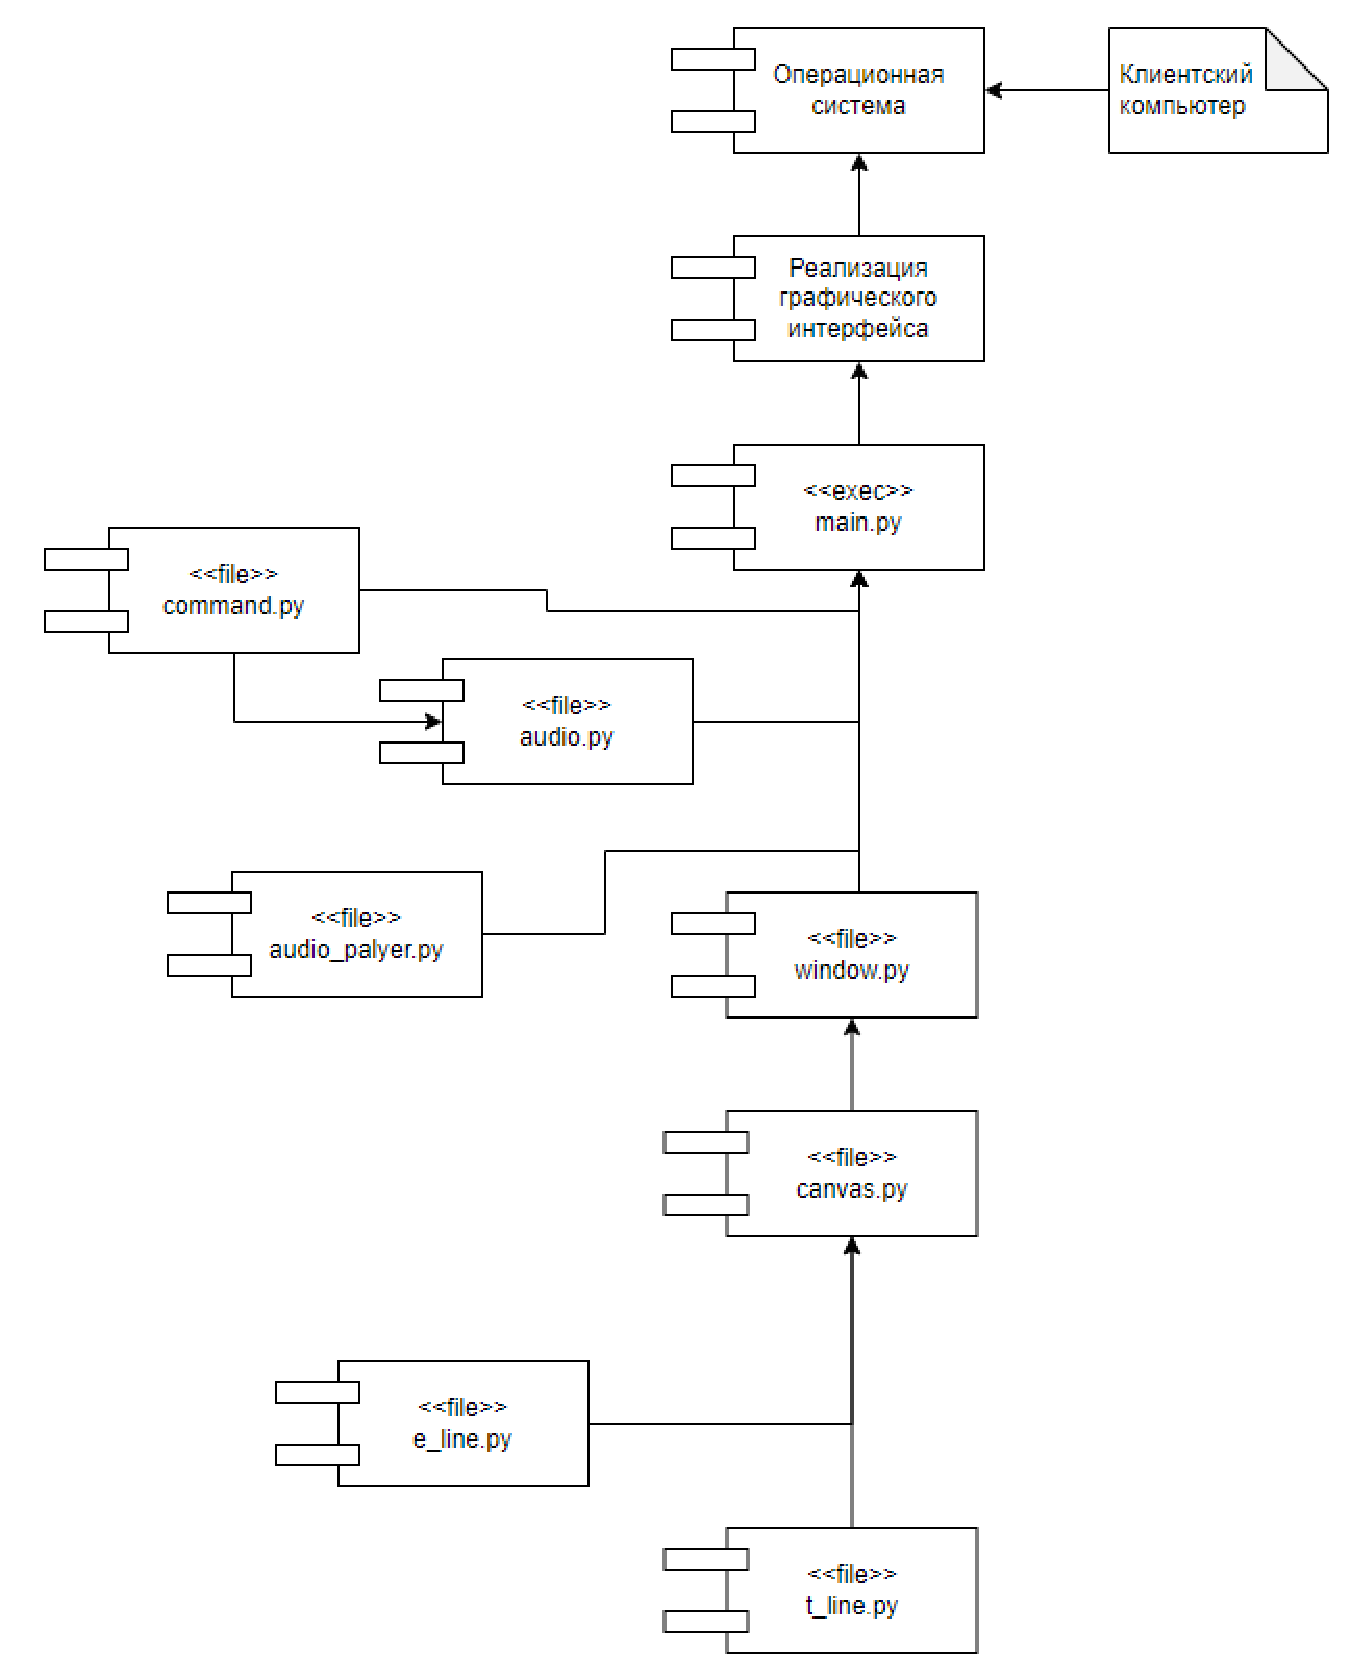
\includegraphics[width=0.7\linewidth]{diagram_comp}}
	\caption{Диаграмма компонентов}
	\label{diagram_comp:image}
\end{figure}

\begin{figure}[ht]
	\center{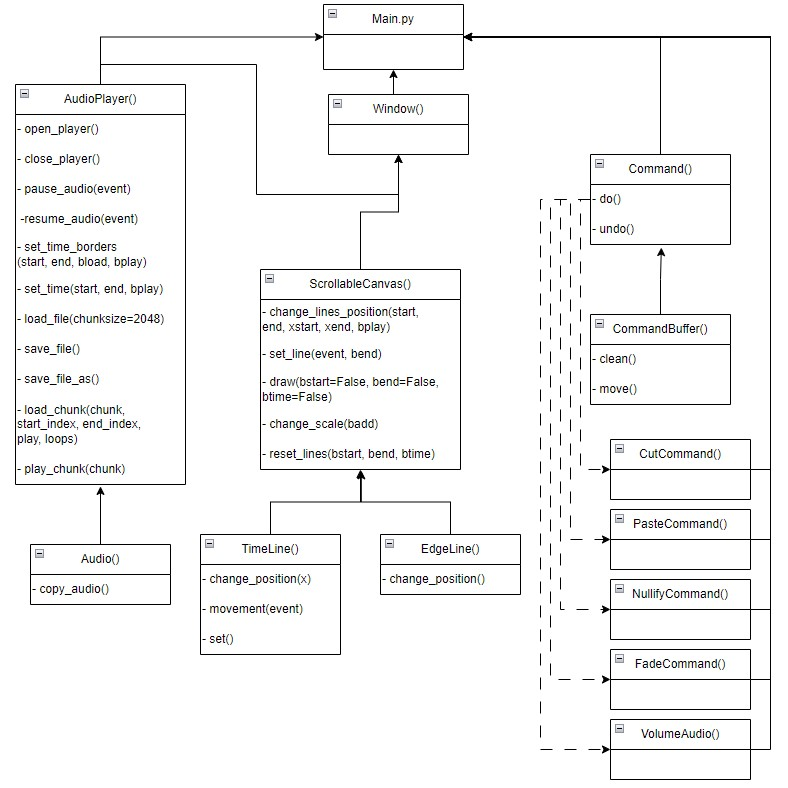
\includegraphics[width=0.9\linewidth]{diagram_class}}
	\caption{Диаграмма классов}
	\label{diagram_class:image}
\end{figure}

Основным исполняемым файлов является файл main.py, объединяющий в себе все другие компоненты. При запуске происходит создание графичексого интерфейса, посредством которого пользователь может взаимодействовать с программой. 